% Causal Inference and Offline RL (thesis_v2 trimmed version)
% Keeps: confounded MDP formalism, causal Bellman operator, naive bias lemma,
% backdoor identification, brief alternative strategies, simulation with figure.

The offline RL algorithms of the preceding section assume that the behavioral policy $\mu$ is a known function of the observed state $s_t$. In many applied settings this assumption fails. A hospital's treatment decisions depend on unobserved patient severity. A firm's pricing depends on private demand signals unavailable to the analyst. When unobserved confounders simultaneously influence both the behavioral policy and the transitions or rewards, standard off-policy evaluation produces biased results, the sequential analogue of omitted variable bias in regression. This section formalizes the problem and reviews identification strategies with direct econometric analogues.

\subsection{The Confounded MDP}
\label{subsec:confounded_mdp}

\citet{zhang2019near}, \citet{zhang2020causal}, and \citet{kallus2020confounding} formalize confounded sequential decision problems using Pearl's do-operator.\footnote{The interventional distribution $P(Y \mid \operatorname{do}(X = x))$ arises when $X$ is set externally rather than observed passively, severing all incoming causal influences on $X$ while leaving the remaining data-generating process intact. The do-operator is formalized within the structural causal model (SCM) framework of \citet{pearl2009causality}.}

\begin{definition}[Confounded MDP {\citep{zhang2020causal}}]
\label{def:confounded_mdp}
A confounded MDP is a tuple $(\mathcal{S}, \mathcal{A}, \mathcal{U}, P, r, \gamma)$ where $\mathcal{U}$ is a space of unobserved confounders and the dynamics are governed by structural equations
\begin{align}
U_t &\sim P_U(\cdot \mid S_t), \label{eq:cmdp_confounder} \\
A_t &\sim \mu(\cdot \mid S_t, U_t), \label{eq:cmdp_action} \\
R_t &= f_R(S_t, A_t, U_t) + \epsilon_t, \label{eq:cmdp_reward} \\
S_{t+1} &\sim f_S(\cdot \mid S_t, A_t, U_t). \label{eq:cmdp_transition}
\end{align}
The behavioral policy $\mu$ depends on the unobserved confounder $U_t$ through Equation~\eqref{eq:cmdp_action}. An evaluation policy $\pi(a \mid s)$ depends only on the observed state.
\end{definition}

Because $\mu$ depends on $U_t$, conditioning on $\{A_t = a\}$ carries information about the confounder, so the observational and interventional transitions diverge: $P(s' \mid s, a) \neq P(s' \mid s, \operatorname{do}(a))$. The Bellman equation for policy evaluation must use interventional, not observational, transition probabilities.

\begin{definition}[Causal Bellman Operator {\citep{zhang2020causal}}]
\label{def:causal_bellman}
The causal Bellman operator $\mathcal{T}_c^\pi$ for policy $\pi$ in a confounded MDP is
\begin{equation}
(\mathcal{T}_c^\pi V)(s) = \sum_{a \in \mathcal{A}} \pi(a \mid s) \sum_{s' \in \mathcal{S}} P(s' \mid s, \operatorname{do}(a)) \bigl[ r(s, a) + \gamma V(s') \bigr],
\label{eq:causal_bellman}
\end{equation}
where $r(s,a) = \mathbb{E}[R_t \mid S_t = s, \operatorname{do}(A_t = a)]$ is the interventional expected reward.
\end{definition}

\begin{lemma}[Bias of Naive Off-Policy Evaluation {\citep{kallus2020confounding}}]
\label{lem:naive_bias}
In a confounded MDP, solving the Bellman equation with observational transitions $P(s' \mid s, a)$ yields $\hat{V}^{\pi}_{\text{naive}}(s) \neq V^\pi(s)$. The importance-sampling estimator using the marginal propensity $\mu(a \mid s)$ rather than the true propensity $\mu(a \mid s, u)$ is also biased.\footnote{This is the sequential analogue of omitted variable bias. In the static case, regressing $Y$ on $X$ without controlling for $U$ yields a biased coefficient. In the sequential case, the bias propagates through the Bellman recursion and can amplify over the horizon.}
\end{lemma}

\subsection{Identification Strategies}

The backdoor criterion \citep{pearl2009causality} provides the primary path to identification.

\begin{theorem}[Backdoor Identification in Confounded MDPs {\citep{pearl2009causality,zhang2020causal}}]
\label{thm:backdoor_mdp}
If observed variables $\mathbf{Z}_t$ block all backdoor paths from $A_t$ to $S_{t+1}$ and no element of $\mathbf{Z}_t$ is a descendant of $A_t$, the interventional transition is identified:
\begin{equation}
P(s' \mid s, \operatorname{do}(a)) = \sum_{\mathbf{z}} P(s' \mid s, a, \mathbf{z}) \, P(\mathbf{z} \mid s).
\label{eq:backdoor_mdp}
\end{equation}
\end{theorem}

Three alternative identification strategies apply when no backdoor variable is available, each with a direct econometric analogue. The front-door criterion \citep{pearl2009causality} identifies causal effects through an observed mediator $M_t$ that intercepts all directed paths from action to outcome, the sequential analogue of mediation analysis. Instrumental variables \citep{liao2024_iv_rl} use an exogenous instrument $Z_t$ satisfying relevance and exclusion to recover the transition function from conditional moment restrictions, directly paralleling two-stage least squares.\footnote{\citet{liao2024_iv_rl} illustrate with NICU assignment, where differential travel time to specialty care is an instrument for admission decisions confounded by unobserved patient severity.} Proximal causal inference \citep{bennett2021proximal} uses two noisy proxy variables for the latent confounder, solving a bridge function equation to recover interventional quantities without ever observing the confounder. For comprehensive surveys of causal RL, including causal representation learning, counterfactual policy optimization, and causal transfer, see \citet{deng2023causal} and \citet{dacostacunha2025unifying}.

\subsection{Simulation Study: Confounded Retail Pricing}
\label{subsec:sim_confounded_ope}

I construct a 5-state engagement funnel with two actions (promote, hold price) and an absorbing conversion state. A retailer manages customers through engagement stages, deciding whether to offer a promotional discount. The data-generating process embeds four distinct sources of causal variation (observed market conditions, unobserved consumer sentiment, an independent cost shock as instrument, and a mediator), enabling simultaneous validation of all four identification strategies from a single DGP.\footnote{Market conditions $Z_t \sim \text{Bernoulli}(0.5)$ satisfy the backdoor criterion. Consumer sentiment $U_t$ is the unobserved confounder, with $P(U_t{=}1 \mid Z_t{=}1) = 0.9$. An independent cost shock is the instrument. Promotions trigger marketing follow-ups $M_t$ as the mediator. Two noisy proxies of $U_t$ (CRM score and browsing behavior) satisfy the proximal conditions. The behavioral policy $\mu(\text{promote} \mid s, U_t, \text{IV}_t) = 0.55 + \rho \cdot 0.25 \cdot (2U_t - 1) + 0.15 \cdot (\text{IV}_t - 0.5)$, where $\rho$ controls confounding strength. Each configuration uses 2,000 trajectories averaged over 20 seeds.}

\begin{figure}[htbp]
\centering
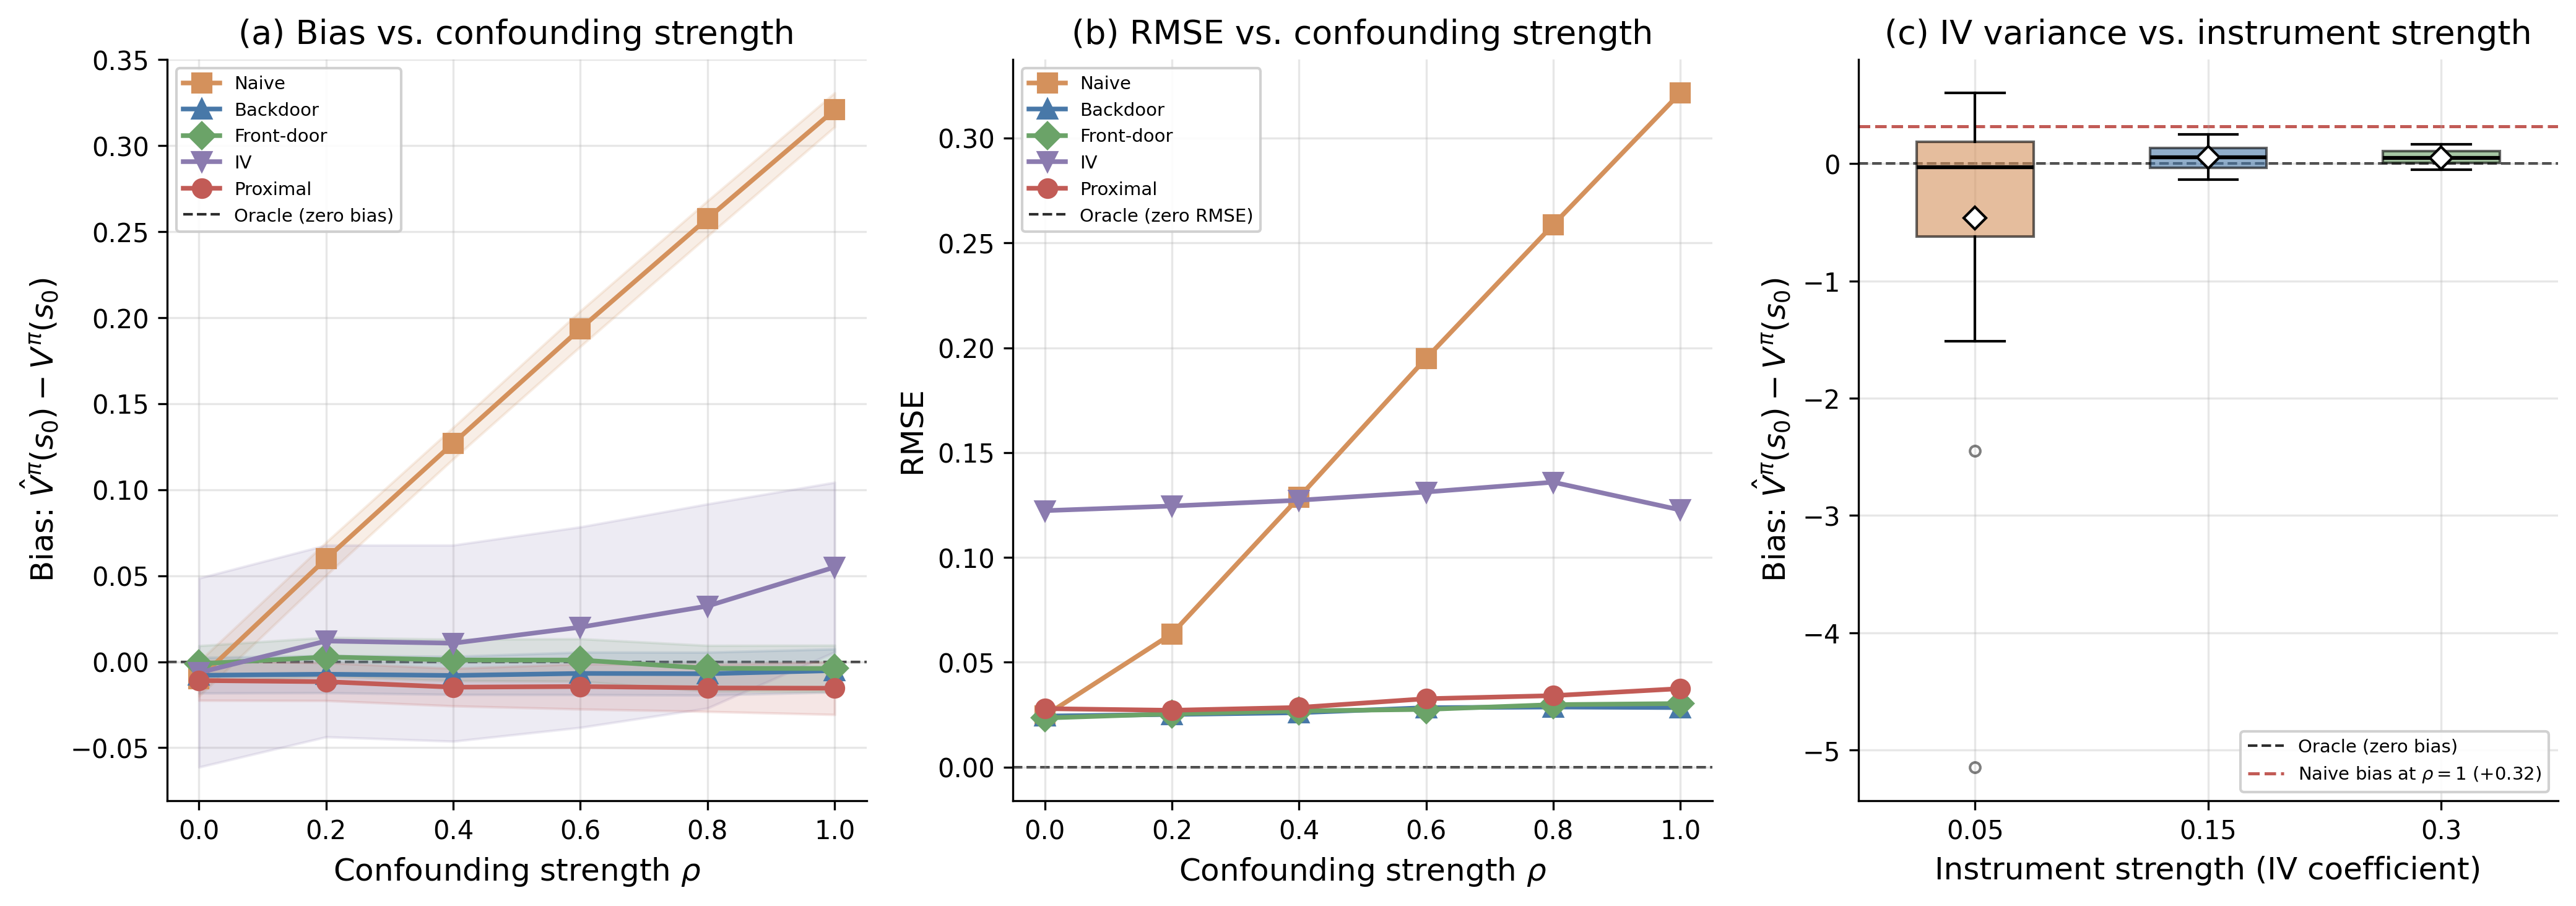
\includegraphics[width=\textwidth]{../ch10_causal/sims/confounded_ope_bias.png}
\caption[Bias and RMSE of OPE estimators under confounding]{\textbf{Bias and RMSE of OPE estimators under confounding.} (a) Bias of five OPE estimators as a function of confounding strength $\rho$. (b) RMSE of five estimators as a function of $\rho$. (c) IV estimator bias distribution vs.\ instrument strength at $\rho = 1$; dashed red line is naive estimator bias.}
\label{fig:confounded_ope}
\end{figure}

The naive estimator's bias grows monotonically with $\rho$ because observational transitions overestimate promotion success. The promote action is more likely when $U_t = 1$, which correlates with favorable conditions, so per-step bias compounds through the Bellman recursion (Figure~\ref{fig:confounded_ope}). The backdoor and front-door estimators eliminate bias at all $\rho$, validating Theorem~\ref{thm:backdoor_mdp}. The IV estimator maintains low bias but higher variance due to the Wald ratio's sensitivity to instrument strength. The proximal estimator achieves low bias with moderate variance, confirming that bridge functions recover causal effects from noisy proxies.
